\section{GPU Prefix-Doubler}
\label{algorithm:gpuprefix}
Mit \currentauthor{Oliver Magiera und\\ Hermann Foot} fortlaufendem Fortschritt in der Entwicklung von General-Purpose-GPUs (GPGPUs), insbesondere innerhalb der letzten Jahre, wurde der Gebrauch von Grafikkarten als Koprozessor für grafikunabhängige Algorithmen immer populärer. Dabei ermöglicht die Bauweise der Grafikprozessoren eine hohe Parallelität und beschleunigt die Berechnungen enorm. Entwicklungsumgebungen wie das NVIDIA CUDA Toolkit werden fortlaufend weiterentwickelt und integrieren vor allem für allgemeine GPU-Berechnungen immer mehr Möglichkeiten. Zusätzlich bieten Libraries wie \textit{Thrust} und \textit{CUB} bereits eine Unterstützung allgemeiner Algorithmen auf der Grafikkarte wie Radixsort oder Präfixsummen an.

Auch im Bereich der Suffix-Array Konstruktionsalgorithmen entstanden für dieses Rechenmodell bereits Ansätze. Dazu gehört unter anderem der Prefix-Doubling Ansatz von Osipov \cite{osipovGPU}, der Skew Ansatz von Deo und Keely \cite{deoGPU} und ein Hybrid beider Varianten von Wang, Baxter und Owens \cite{wangGPU}. Im Rahmen unserer Projektgruppe haben wir uns auf ersteren fokussiert und diesen innerhalb des Frameworks implementiert und evaluiert.

In diesem Kapitel werden wir dazu zunächst den sequentiellen Algorithmus von Osipov vorstellen und an einem Beispiel erläutern, bevor wir auf die Ideen der Parallelisierung und deren Implementierungen, speziell im Bezug auf die GPU, eingehen.

\subsection{Algorithmus}
Die Idee des Algorithmus von Osipov basiert sowohl auf den Prefix-Doublern von Larson und Sadakane \cite{saca:1}, als auch von Manber und Myers \cite{Manber1993}. In Bezug auf Parallelität hat Ersterer das Problem, dass die zu sortierenden Gruppen innerhalb einer Iteration unterschiedliche Längen haben können, wodurch unbalancierte Workloads entstehen. Der Algorithmus von Manber und Myers dagegen hat dieses Problem zwar nicht, sortiert dafür aber bereits fertig sortierte Suffixe erneut. Die Idee ist es nun, beide Ansätze zu kombinieren, also global zu sortieren, allerdings nur mit den Suffixen, die noch nicht fertig sortiert wurden oder für die Sortierung noch benötigt werden. Dabei soll folgendes Lemma helfen:
\begin{lemma}\label{lem:sort-gruppe}
Falls in der i-ten Iteration des Manber-Myers Algorithmus gilt, dass
\begin{itemize}
\item $\mathsf{S}_i$ ist eine sortierte Gruppe in $\mathsf{SA}_{2^k}$
\item $i < 2^{k+1}$ oder $\mathsf{S}_{i-2^{k+1}}$ ist eine sortierte Gruppe
\end{itemize} 
dann gilt für alle nachfolgenden Iterationen $j>k$ entweder $i<2^i$ oder $\mathsf{S}_{i-2^j}$ ist eine sortierte Gruppe.
\end{lemma}
% Beispiel?
Es besagt, dass sortierte Gruppen, welche im nächsten Schritt eine bereits sortierte Gruppe sortieren würden, nicht mehr betrachtet werden müssen. Dies ist möglich, da durch die Verdopplung der betrachteten Suffixlänge das hintere der beiden Suffixe immer wieder Gruppen sortieren würde, welche bereits durch seinen Vorgänger sortiert wurden.
Mit Hilfe dieses Lemmas können wir nun, falls die Bedingungen zutreffen, fertig sortierte Gruppen innerhalb des Sortierschritt nicht weiter beachten, um redundante Arbeit zu vermeiden.

\begin{listing}
\begin{minted}[escapeinside=||,mathescape=true,numbers=left]{python}
osipov(T)
# Tupel = ($\mathsf{SA}_{2h}$, $h$-rank, $2h$-rank)
 Sort suffixes |$\mathsf{S}_i$| according to their first four characters |in| |$\mathsf{SA}_4$| 
 Init |$\mathsf{ISA}_4$| 
 Mark sorted Groups |in| |$\mathsf{ISA}_4$| by negation
 |$size = n, h = 4$| 
 while |$(size > 0)$|:  
   |$s = 0$|
   for |$j$| in |$[0, size]$|:
      |$i = \mathsf{SA}_h[j]-h$|
      if |$((i>0) \land (\mathsf{ISA}_h[i]>0))$|:
         triples.add|$((i, \mathsf{ISA}_h[i], \mathsf{ISA}_h[\mathsf{SA}_h[j]]))$|
         |$s$|++
      |$i = \mathsf{SA}_h[j]$|
      if |$((\mathsf{ISA}_h[i]<0) \land (i-2h\geq 0) \land (\mathsf{ISA}_h[i-2h] \geq 0))$|:
         triples.add|$((i, \mathsf{ISA}_h[i], -\mathsf{ISA}_h[i]))$|
         |$s$|++
    sort|$($\text{value}$(\mathsf{SA}_{2h},2h\text{-rank})$|, key|$(h\text{-rank}))$|
    |$head = 0$|
    for |$j$| in |$[1,s]$|:
       if |$(h\text{-rank}[j] > h\text{-rank}[head])$|:
          |$head = j$|
       else:
          if |$(2h\text{-rank}[j] \neq 2h\text{-rank}[head])$|:
             |$h\text{-rank}[j]= h\text{-rank}[head]+j-head$|
             |$head=j$|
          else:
             |$h\text{-rank}[j]= h\text{-rank}[head]$|
    for |$i$| in |$[0,s]$|:
       |$\mathsf{ISA}_{2h}[\mathsf{SA}_{2h}[i]]=h\text{-rank}[\mathsf{SA}_{2h}[i]]$|
    Mark sorted Groups |in| |$\mathsf{ISA}_{2h}$| by negation
    |$size=s, h = 2 \cdot h$| 
 Calculate |$\mathsf{SA}\ \text{from}\ \mathsf{ISA}_h$|
\end{minted}
\caption{Der sequentielle Prefix-Doubling Algorithmus von Osipov.}
\label{alg:osipov}
\end{listing}

In Algorithmus \ref{alg:osipov} können wir den Ablauf des Prefix-Doublers von Osipov sehen. In der ersten Zeile werden die Suffixe anhand ihrer ersten vier Zeichen sortiert und die daraus resultierende Reihenfolge in $\mathsf{SA}_4$ gespeichert. Darauf aufbauend wird das $\mathsf{ISA}_4$ konstruiert, darin bereits fertig sortierte Elemente mit einem Flag markiert und die Variablen $size$ und $h$ initialisiert. Die folgende Schleife wird solange wiederholt, bis sich alle Elemente in sortierten Gruppen befinden. Nach der finalen Sortierung müssen wir noch das finale $\mathsf{SA}$ aus dem finalen $\mathsf{ISA}$ erzeugen.

Für die Sortierung eines Schleifendurchlaufes müssen wir zunächst die benötigten Tupel erzeugen. Dafür prüfen wir in Z.~9, ob wir das Suffix $\mathsf{S}_i$ mit dem Suffix $\mathsf{S}_j$ induzieren können, d.~h.\ $i = \mathsf{SA}_{h}[j]-h$ ist ein gültiger Index und wir haben $\mathsf{S}_i$ noch nicht endgültig sortiert. Ist dieser Fall gegeben, erzeugen wir in Z.~10 \ das Tupel aus dem Suffxindex $i$, seinem $h$-Rang $\mathsf{ISA}_h[i]$ sowie seinem $2h$-Rang $\mathsf{ISA}_h[\mathsf{SA}_h[j]]$, welcher dem Rang des Suffixes $\mathsf{S}_j$ entspricht. Als nächstes prüfen wir, ob unser Suffix $\mathsf{S}_j$ für die folgenden Iterationen weiterhin benötigt wird (s.~Lemma \ref{lem:sort-gruppe}). Ist dies der Fall, so erzeugen wir das Tupel in Z.~14 aus dem Index, dem negierten Rang und dem Rang des Suffixes $\mathsf{S}_j$. Für jedes erzeugte Tupel erhöhen wir $s$ um eins. $s$ entspricht somit der Anzahl an Tupeln und damit der Anzahl an Suffixen in $\mathsf{SA}_{2h}$.

Um die neuen Ränge bestimmen zu können, müssen wir unsere Tupel zunächst stabil sortieren (Z.~16). Als Sortierschlüssel wählen wir hierbei den $h$-Rang. Daraufhin durchlaufen wir jedes Suffix in $\mathsf{SA}_{2h}$ und berechnen den neuen Rang. Ist der Rang des aktuell betrachteten Suffixes $\mathsf{S}_j$ größer als der Rang des aktuellen Kopfes, haben wir eine neue Gruppe gefunden (Z.~19) und setzen den Kopf auf den Anfang der neuen Gruppe. Andernfalls prüfen wir, ob das betrachtete Suffix $j$ einen anderen $2h$-Rang hat als der aktuelle Kopf. In diesem Fall haben wir eine neue Gruppe durch die aktuelle Iteration und die Suffix-Länge $2h$ erhalten und können diese Suffixe zum ersten Mal eindeutig voneinander unterscheiden. Dafür setzen wir den Rang auf den Rang des Kopfes und addieren die Differenz der Positionen in $\mathsf{SA}_{2h}$ zwischen Suffix $j$ und dem Kopf drauf. Sollten sowohl die $h$- als auch die $2h$-Ränge identisch sein, können wir die Suffixe noch nicht eindeutig unterscheiden und wir weisen $\mathsf{S}_j$ den Rang des Kopfes zu (Z.~26), da sich dessen Rang durch eine neue Gruppe in dieser Iteration verändert haben könnte (Z.~22--24).

Zum Abschluss der Iteration müssen wir die neuen Ränge in $\mathsf{ISA}_{2h}$ schreiben (Z.~27f.) und alle neuen, vollständig sortierten Gruppen mittels Negierung markieren (Z.~29). Die neue Größe für die nächste Iteration entspricht der Anzahl Tupel dieser Iteration und $h$ wird für den nächsten Schleifendurchlauf verdoppelt (Z.~30).

% Beispiel für kompletten Algorithmus
\subsection{Beispiel}
% Please add the following required packages to your document preamble:
% \usepackage{multirow}
\begin{table}[]
\small
\begin{tabular}{|l|l|l|l|l|l|l|l|l|l|l|l|l|l|l|l|}
\hline
$j$                                                                          & 0  & 1  & 2 & 3 & 4  & 5 & 6 & 7 & 8  & 9 & 10 & 11 & 12 & 13 & 14 \\ \hline
$\mathsf{SA}[j]$                                                                  & 14 & 13 & 1 & 7 & 12 & 2 & 8 & 4 & 10 & 3 & 9  & 0  & 6  & 11 & 5  \\ \hline
\multirow{2}{*}{\begin{tabular}[c]{@{}l@{}}Suffix \\ $h=2$ \end{tabular}} & \$ & a  & a & a & a  & a & a & a & a  & b & b  & c  & c  & c  & c  \\
                                                                           &    & \$ & a & a & a  & b & b & c & c  & a & a  & a  & a  & a  & c  \\ \hline
$\mathsf{ISA}[\mathsf{SA}[j]]$                                                         & -0 & -1 & 2 & 2 & 2  & 5 & 5 & 7 & 7  & 9 & 9  & 11 & 11 & 11 & -14 \\ \hline
\end{tabular}
\caption{Schritte vor dem Schleifendurchlauf: initiale Sortierung nach den ersten $h$-Zeichen (hier: $h=2$), initiales $\mathsf{ISA}$ (in $\mathsf{SA}$-Reihenfolge) und Markierung bereits sortierter Gruppen}
\label{tab:osipov-init}
\end{table}


Im Folgenden gehen wir auf das bekannte Beispiel \glqq caabaccaabacaa\$\grqq ~ein, um die Funktionsweise des Prefix-Doublers nach Osipov zu veranschaulichen. Um möglichst viele Schritte bzw.\ Verzweigungen darzustellen, setzen wir die initiale Länge der Suffixe auf $h=2$ statt auf $4$.

Zunächst sortieren wir unsere Suffixe nach den ersten zwei Zeichen und erzeugen basierend darauf das initiale $\mathsf{ISA}_2$. Die Ränge bereits sortierter Gruppen werden negiert, so wie bei den Suffixen mit Index $14, 13 ~\text{und}~ 5$ zu sehen. Die Ergebnisse dieser drei Schritte sind in Tabelle \ref{tab:osipov-init} dargestellt. Als nächstes betrachten wir die erste Iteration unserer Schleife. 

\begin{table}[]
\small
\begin{tabular}{|l|l|l|l|l|}
\hline
$j$ & $i = \mathsf{SA}_h[j] - h$ & $i > 0 \wedge \mathsf{ISA}_h[i] > 0$ & $i' = \mathsf{SA}_h[j]$ & \begin{tabular}[c]{@{}l@{}}$\mathsf{ISA}_h[i'] < 0$\\ $\wedge (i' - 2h) \geq 0$ \\ $\wedge ~\mathsf{ISA}_h[i' - 2h] \geq 0$\end{tabular} \\ \hline
0   & 12              & $\top \wedge \top = \top$   & 14           & $\top \wedge \top \wedge \top = \top$                                                                                             \\ \hline
1   & 11              & $\top \wedge \top = \top$   & 13           & $\top \wedge \top \wedge \top = \top$                                                                                             \\ \hline
2   & -1              & $\bot$                      & 1            & $\bot$                                                                                                                            \\ \hline
3   & 5               & $\top \wedge \bot = \bot$          & 7            & $\bot$                                                                                                                            \\ \hline
4   & 10              & $\top \wedge \top = \top$   & 12           & $\bot$                                                                                                                            \\ \hline
5   & 0               & $\top \wedge \top = \top$   & 2            & $\bot$                                                                                                                            \\ \hline
6   & 6               & $\top \wedge \top = \top$   & 8            & $\bot$                                                                                                                            \\ \hline
7   & 2               & $\top \wedge \top = \top$   & 4            & $\bot$                                                                                                                            \\ \hline
8   & 8               & $\top \wedge \top = \top$   & 10           & $\bot$                                                                                                                            \\ \hline
9   & 1               & $\top \wedge \top = \top$   & 3            & $\bot$                                                                                                                            \\ \hline
10  & 7               & $\top \wedge \top = \top$   & 9            & $\bot$                                                                                                                            \\ \hline
11  & -2              & $\bot$                      & 0            & $\bot$                                                                                                                            \\ \hline
12  & 4               & $\top \wedge \top = \top$   & 6            & $\bot$                                                                                                                            \\ \hline
13  & 9               & $\top \wedge \top = \top$   & 11           & $\bot$                                                                                                                            \\ \hline
14  & 3               & $\top \wedge \top = \top$   & 5            & $\top \wedge \top \wedge \top = \top$                                                                                             \\ \hline
\end{tabular}
\caption{Bedingungen für die Erzeugung von Tupeln für $h=2$. Die erste Bedingung (zweite Spalte) prüft, ob der Suffix-Index sortiert werden muss. Die zweite Bedingung (vierte Spalte) prüft, ob bereits sortierte Suffixe zum Sortieren anderer Suffixe in den Folgeiterationen benötigt werden (s. Lemma \ref{lem:sort-gruppe}).}
\label{tab:osipov-tupel-cond}
\end{table}

Zu Beginn einer jeden Iteration müssen wir die für die Sortierung benötigten Tupel erzeugen. Dafür schauen wir uns zunächst an, welche Tupel überhaupt benötigt werden. Tabelle \ref{tab:osipov-tupel-cond} listet den Index $j$ der inneren Schleife, den korrespondierenden Suffix-Index $\mathsf{SA}_h[j]-h$ und die Bedingung zur Erzeugung des Tupels. Dabei muss $i>0$ auf einen gültigen Index zeigen, dessen Suffix noch nicht eindeutig sortiert sein darf ($\mathsf{ISA}_h[i] > 0$). Ebenso haben wir den Suffix-Index $\mathsf{SA}_h[j]$ sowie die entsprechende Bedingung notiert. Die Bedingung entspricht hierbei der Negierung von Lemma \ref{lem:sort-gruppe}. Die Bedingungen sind als Lazy Evaluation dargestellt, d.~h.\ sobald ein Wert $\mathsf{false}$ ist, schreiben wir die Auswertung der weiteren Teilbedingungen nicht auf. In der ersten Iteration werden alle Suffixe außer $S_0 ~\text{und}~ S_1$ zum Erzeugen neuer Tupel verwendet. Wir erzeugen durch die zweite Bedingung darüber hinaus Tupel mit den Suffixen mit Index $14, 13 ~\text{und}~ 5$, da wir sie möglicherweise für die nächste Iteration zum weiteren Sortieren benötigen.

\begin{table}[]
\small
\begin{tabular}{|l|l|l|}
\hline
Erzeugte Tupel & $j$  & Sortierte Reihenfolge (nach $h$-Rang) \\ \hline
$(12, 2, -0)$  & 0  & $(14,0,-0)$                           \\ \hline
$(14, 0, -0)$  & 1  & $(13,1,-1)$                           \\ \hline
$(11,11,-1)$   & 2  & $(12,2,-0)$                           \\ \hline
$(13,1,-1)$    & 3  & $(1,2,9)$                             \\ \hline
$(10,7,2)$     & 4  & $(7,2,9)$                             \\ \hline
$(0,11,5)$     & 5  & $(2,5,7)$                             \\ \hline
$(6,11,5)$     & 6  & $(8,5,7)$                             \\ \hline
$(2,5,7)$      & 7  & $(10,7,2)$                            \\ \hline
$(8,5,7)$      & 8  & $(4,7,11)$                            \\ \hline
$(1,2,9)$      & 9  & $(9,9,11)$                            \\ \hline
$(7,2,9)$      & 10 & $(3,9,-14)$                           \\ \hline
$(4,7,11)$     & 11 & $(11,11,-1)$                          \\ \hline
$(9,9,11)$     & 12 & $(0,11,5)$                            \\ \hline
$(3,9,-14)$    & 13 & $(6,11,5)$                            \\ \hline
$(5,14,-14)$   & 14 & $(5,14,-14)$                          \\ \hline
\end{tabular}
\caption{Die erzeugten Tupel (erste Spalte) in der Reihenfolge aus Tabelle \ref{tab:osipov-tupel-cond}, sowie in nach dem $h$-Rang sortierter Reihenfolge (dritte Spalte) und dem entsprechenden Tupelindex $j$.}
\label{tab:osipov-tupel-sort}
\end{table}

Die erzeugten Tupel und die daraus resultierende Sortierung sind in Tabelle \ref{tab:osipov-tupel-sort} dargestellt. Dort sehen wir für die Suffix-Indizes $14, 13 ~\text{sowie}~ 5$, dass ihnen ihr $\mathsf{ISA}_2$ Wert als $2h$-Rang und dessen Negierung als $h$-Rang zugewiesen wurden. Wichtig hierbei ist, dass für die zweite Komponente, den $h$-Rang, nur positive Werte gespeichert werden, damit die folgende Sortierung die Reihenfolge bereits sortierter Suffixe nicht verändert. Die dritte Komponente dient bei den drei bereits sortierten Suffixen nur als Platzhalter. Bei den übrigen Suffixen dient dieser Wert als finale Unterscheidungsmöglichkeit für die resultierende Sortierung. Da dabei auf Ungleichheit geprüft wird, stellen negative Werte, wie für die Suffix-Indizes $3, 11$ oder $12$, kein Problem dar. Nach der Erzeugung und Sortierung der Tupel können wir im nächsten Schritt die neuen Ränge berechnen.

\iffalse
% Please add the following required packages to your document preamble:
% \usepackage[table,xcdraw]{xcolor}
% If you use beamer only pass "xcolor=table" option, i.e. \documentclass[xcolor=table]{beamer}
\begin{table}[]
\small
\begin{tabular}{|c|c|c|c|c|c|}
\hline
Indizes                                                    & \begin{tabular}[c]{@{}c@{}}$h\text{-rank}[j] >$\\ $h\text{-rank}[head]$\end{tabular}                                      & \begin{tabular}[c]{@{}c@{}}$2h\text{-rank}[j] \neq$\\ $2h\text{-rank}[head]$\end{tabular}                                      & \begin{tabular}[c]{@{}c@{}}$h\text{-rank}[j]=$\\ $h\text{-rank}[head]$\\ $+ j - head$ \\ (neue Gruppe)\end{tabular} & \begin{tabular}[c]{@{}c@{}}$h\text{-rank}[j]=$\\ $h\text{-rank}[head]$\\ (Rang \\ übernehmen)\end{tabular} & \begin{tabular}[c]{@{}c@{}}$head$ \\ (neuer Wert)\end{tabular} \\ \hline
\begin{tabular}[c]{@{}c@{}}$head=2$\\ $j=3$\end{tabular}   & \begin{tabular}[c]{@{}c@{}}$h\text{-rank}[3] = 2$\\ $= h\text{-rank}[2]$\end{tabular}                                     & \cellcolor[HTML]{3166FF}\begin{tabular}[c]{@{}c@{}}$2h\text{-rank}[3]$\\ $= 9 \neq -0$\\ $= 2h\text{-rank}[2]$\end{tabular}    & \cellcolor[HTML]{32CB00}\begin{tabular}[c]{@{}c@{}}$h\text{-rank}[3]$\\ $=2 + 3 - 2$\\ $= 3$\end{tabular}           & -                                                                                                          & $head = 3$                                                     \\ \hline
\begin{tabular}[c]{@{}c@{}}$head=3$\\ $j=4$\end{tabular}   & \begin{tabular}[c]{@{}c@{}}$h\text{-rank}[4]$\\ $= 2 < 3$\\ $= h\text{-rank}[3]$\end{tabular}                             & \begin{tabular}[c]{@{}c@{}}$2h\text{-rank}[4] = 9$\\ $= 2h\text{-rank}[3]$\end{tabular}                                        & -                                                                                                                   & \begin{tabular}[c]{@{}c@{}}$h\text{-rank}[4]$\\ $=h\text{-rank}[3]$\\ $= 3$\end{tabular}                   & -                                                              \\ \hline
\begin{tabular}[c]{@{}c@{}}$head=3$\\ $j=5$\end{tabular}   & \cellcolor[HTML]{3166FF}\begin{tabular}[c]{@{}c@{}}$h\text{-rank}[5]$\\ $= 5 > 3$\\ $= h\text{-rank}[3]$\end{tabular}     & -                                                                                                                              & -                                                                                                                   & -                                                                                                          & $head = 5$                                                     \\ \hline
\begin{tabular}[c]{@{}c@{}}$head=5$\\ $j=6$\end{tabular}   & \begin{tabular}[c]{@{}c@{}}$h\text{-rank}[6] = 5$\\ $= h\text{-rank}[5]$\end{tabular}                                     & \begin{tabular}[c]{@{}c@{}}$2h\text{-rank}[6] = 7$\\ $= 2h\text{-rank}[5]$\end{tabular}                                        & -                                                                                                                   & \begin{tabular}[c]{@{}c@{}}$h\text{-rank}[6]$\\ $=h\text{-rank}[5]$\\ (Rang \\ unverändert)\end{tabular}   & -                                                              \\ \hline
\begin{tabular}[c]{@{}c@{}}$head=5$\\ $j=7$\end{tabular}   & \cellcolor[HTML]{3166FF}\begin{tabular}[c]{@{}c@{}}$h\text{-rank}[7]$\\ $= 7 >5$\\ $= h\text{-rank}[5]$\end{tabular}      & -                                                                                                                              & -                                                                                                                   & -                                                                                                          & $head=7$                                                       \\ \hline
\begin{tabular}[c]{@{}c@{}}$head=7$\\ $j=8$\end{tabular}   & \begin{tabular}[c]{@{}c@{}}$h\text{-rank}[8] = 7$\\ $= h\text{-rank}[7]$\end{tabular}                                     & \cellcolor[HTML]{3166FF}\begin{tabular}[c]{@{}c@{}}$2h\text{-rank}[8]$\\ $= 11 \neq 2$\\ $= 2h\text{-rank}[7]$\end{tabular}    & \cellcolor[HTML]{32CB00}\begin{tabular}[c]{@{}c@{}}$h\text{-rank}[8]$\\ $= 7 + 8 - 7$\\ $= 8$\end{tabular}          & -                                                                                                          & $head=8$                                                       \\ \hline
\begin{tabular}[c]{@{}c@{}}$head=8$\\ $j=9$\end{tabular}   & \cellcolor[HTML]{3166FF}\begin{tabular}[c]{@{}c@{}}$h\text{-rank}[9]$\\ $= 9 > 8$\\ $= h\text{-rank}[8]$\end{tabular}     & -                                                                                                                              & -                                                                                                                   & -                                                                                                          & $head=9$                                                       \\ \hline
\begin{tabular}[c]{@{}c@{}}$head=9$\\ $j=10$\end{tabular}  & \begin{tabular}[c]{@{}c@{}}$h\text{-rank}[10] = 9$\\ $= h\text{-rank}[9]$\end{tabular}                                    & \cellcolor[HTML]{3166FF}\begin{tabular}[c]{@{}c@{}}$2h\text{-rank}[10]$\\ $= -14 \neq 11$\\ $= 2h\text{-rank}[9]$\end{tabular} & \cellcolor[HTML]{32CB00}\begin{tabular}[c]{@{}c@{}}$h\text{-rank}[10]$\\ $= 9 + 10 - 9$\\ $= 10$\end{tabular}       & -                                                                                                          & $head=10$                                                      \\ \hline
\begin{tabular}[c]{@{}c@{}}$head=10$\\ $j=11$\end{tabular} & \cellcolor[HTML]{3166FF}\begin{tabular}[c]{@{}c@{}}$h\text{-rank}[11]$\\ $= 11 > 10$\\ $= h\text{-rank}[10]$\end{tabular} & -                                                                                                                              & -                                                                                                                   & -                                                                                                          & $head=11$                                                      \\ \hline
\begin{tabular}[c]{@{}c@{}}$head=11$\\ $j=12$\end{tabular} & \begin{tabular}[c]{@{}c@{}}$h\text{-rank}[12] = 11$\\ $= h\text{-rank}[11]$\end{tabular}                                  & \cellcolor[HTML]{3166FF}\begin{tabular}[c]{@{}c@{}}$2h\text{-rank}[12]$\\ $= 5 \neq -1$\\ $= 2h\text{-rank}[11]$\end{tabular}  & \cellcolor[HTML]{32CB00}\begin{tabular}[c]{@{}c@{}}$h\text{-rank}[12]$\\ $= 11 + 12 - 11$\\ $=12$\end{tabular}      & -                                                                                                          & $head=12$                                                      \\ \hline
\begin{tabular}[c]{@{}c@{}}$head=12$\\ $j=13$\end{tabular} & \begin{tabular}[c]{@{}c@{}}$h\text{-rank}[13]$\\ $= 11 < 12$\\ $= h\text{-rank}[12]$\end{tabular}                         & \begin{tabular}[c]{@{}c@{}}$2h\text{-rank}[13] = 5$\\ $= 2h\text{-rank}[12]$\end{tabular}                                      & -                                                                                                                   & \begin{tabular}[c]{@{}c@{}}$h\text{-rank}[13]$\\ $=h\text{-rank}[12]$\\ $=12$\end{tabular}                 &                                                                \\ \hline
\end{tabular}
\end{table}
\fi

% Please add the following required packages to your document preamble:
% \usepackage[table,xcdraw]{xcolor}
% If you use beamer only pass "xcolor=table" option, i.e. \documentclass[xcolor=table]{beamer}
\begin{table}[]
\small
\begin{tabular}{|c|c|c|c|c|}
\hline
Indizes                                                    & \begin{tabular}[c]{@{}c@{}}$h\text{-rank}[j] >$\\ $h\text{-rank}[head]$\end{tabular} & \begin{tabular}[c]{@{}c@{}}$2h\text{-rank}[j] \neq$\\ $2h\text{-rank}[head]$\end{tabular} & \begin{tabular}[c]{@{}c@{}}$h\text{-rank}[j]=$\\ $h\text{-rank}[head]$\\ $+ j - head$ \\ (neue Gruppe)\end{tabular} & \begin{tabular}[c]{@{}c@{}}$h\text{-rank}[j]=$\\ $h\text{-rank}[head]$\\ (Rang \\ übernehmen)\end{tabular} \\ \hline
\begin{tabular}[c]{@{}c@{}}$head=2$\\ $j=3$\end{tabular}   & $2 = 2$                                                                              & \cellcolor[HTML]{3166FF}$9 \neq -0$                                                       & \begin{tabular}[c]{@{}c@{}}$h\text{-rank}[3]$\\ $=2 + 3 - 2$\\ $= 3$\end{tabular}                                   & -                                                                                                                               \\ \hline
\begin{tabular}[c]{@{}c@{}}$head=3$\\ $j=4$\end{tabular}   & $2 < 3$                                                                              & $9 = 9$                                                                                   & -                                                                                                                   & \cellcolor[HTML]{32CB00}\begin{tabular}[c]{@{}c@{}}$h\text{-rank}[4]$\\ $=h\text{-rank}[3]$\\ $= 3$\end{tabular}                \\ \hline
\begin{tabular}[c]{@{}c@{}}$head=3$\\ $j=5$\end{tabular}   & \cellcolor[HTML]{3166FF}$5 > 3$                                                      & -                                                                                         & -                                                                                                                   & -                                                                                                                                \\ \hline
\begin{tabular}[c]{@{}c@{}}$head=5$\\ $j=6$\end{tabular}   & $5 = 5$                                                                              & $7 = 7$                                                                                   & -                                                                                                                   & \cellcolor[HTML]{32CB00}\begin{tabular}[c]{@{}c@{}}$h\text{-rank}[6]$\\ $=h\text{-rank}[5]$\\ (Rang \\ unverändert)\end{tabular} \\ \hline
\begin{tabular}[c]{@{}c@{}}$head=5$\\ $j=7$\end{tabular}   & \cellcolor[HTML]{3166FF}$7 > 5$                                                      & -                                                                                         & -                                                                                                                   & -                                                                                                                                \\ \hline
\begin{tabular}[c]{@{}c@{}}$head=7$\\ $j=8$\end{tabular}   & $7 = 7$                                                                              & \cellcolor[HTML]{3166FF}$11 \neq 2$                                                       & \begin{tabular}[c]{@{}c@{}}$h\text{-rank}[8]$\\ $= 7 + 8 - 7$\\ $= 8$\end{tabular}                                  & -      \\ \hline
\begin{tabular}[c]{@{}c@{}}$head=8$\\ $j=9$\end{tabular}   & \cellcolor[HTML]{3166FF}$9 > 8$                                                      & -                                                                                         & -                                                                                                                   & -                                                                                                                                \\ \hline
\begin{tabular}[c]{@{}c@{}}$head=9$\\ $j=10$\end{tabular}  & $9 = 9$                                                                              & \cellcolor[HTML]{3166FF}$-14 \neq 11$                                                     & \begin{tabular}[c]{@{}c@{}}$h\text{-rank}[10]$\\ $= 9 + 10 - 9$\\ $= 10$\end{tabular}                               & -      \\ \hline
\begin{tabular}[c]{@{}c@{}}$head=10$\\ $j=11$\end{tabular} & \cellcolor[HTML]{3166FF}$11 > 10$                                                    & -                                                                                         & -                                                                                                                   & -  \\ \hline
\begin{tabular}[c]{@{}c@{}}$head=11$\\ $j=12$\end{tabular} & $11 = 11$                                                                            & \cellcolor[HTML]{3166FF}$5 \neq -1$                                                       & \begin{tabular}[c]{@{}c@{}}$h\text{-rank}[12]$\\ $= 11 + 12 - 11$\\ $=12$\end{tabular}                              & -                                                                                                                                \\ \hline
\begin{tabular}[c]{@{}c@{}}$head=12$\\ $j=13$\end{tabular} & $11 < 12$                                                                            & $5 = 5$                                                                                   & -                                                                                                                   & \cellcolor[HTML]{32CB00}\begin{tabular}[c]{@{}c@{}}$h\text{-rank}[13]$\\ $=h\text{-rank}[12]$\\ $=12$\end{tabular}               \\ \hline
\end{tabular}
\caption{Neuberechnung der Ränge mittels Tupeln aus Tabelle \ref{tab:osipov-tupel-sort}. Die erste Bedingung (zweite Spalte) prüft, ob eine neue $h$-Gruppe beginnt. Die zweite Bedingung (dritte Spalte) prüft, ob eine neue $2h$-Gruppe beginnt. Ist dies der Fall, muss der neue Rang berechnet werden. Falls die zweite Bedingung nicht erfüllt ist, so wird der Rang des Gruppenkopfes übernommen, in unserem Beispiel grün markiert. Sobald eine neue $h$- oder $2h$-Gruppe beginnt, muss der $head$-Zeiger auf den Anfang der neuen Gruppe zeigen. Ist eine der beiden Bedingungen erfüllt, so wird sie blau markiert.}
\label{tab:osipov-new-ranks}
\end{table}

Tabelle \ref{tab:osipov-new-ranks} zeigt die Berechnung der neuen Ränge. Die ersten beiden Bedingungen prüfen, ob sich die zu vergleichenden Tupel in derselben Gruppe befinden. Bei Ungleichheit der ersten Bedingung $h\text{-rank}[j] > h\text{-rank}[head]$ befinden sich die beiden Suffixe bereits in unterschiedlichen $h$-Gruppen. Bei der zweiten Bedingung $2h\text{-rank}[j] \neq 2h\text{-rank}[head]$ hingegen entsteht eine neue $2h$-Gruppe, da sie sich durch die Verdopplung des Suffixes zum ersten Mal unterscheiden. In diesem Fall muss der neue Rang berechnet werden. Dies geschiet in der $4.$ Spalte. Die blauen Markierungen in den Spalten $2$ und $3$ geben an, dass eine neue Gruppe beginnt, d.~h. die Bedingung ist erfüllt. Wenn keine der beiden Bedingungen gilt, so befinden sich die Suffixe immer noch in derselben Gruppe. Dabei müssen wir den Rang des Gruppenkopfes übernehmen, da sich in der Zwischenzeit der Rang dieser Gruppe erhöht haben könnte. Um dies hervorzuheben, werden die Zuweisungen in der $5.$ Spalte grün markiert. Dies ist beispielsweise für die Gruppe $(1,7)$ (Tupel $3$ und $4$) der Fall, wobei dem Index $1$ im vorigen Durchlauf dieser Schleife der Rang $3$ zugewiesen und somit der Rang $2$ überschrieben wurde. 


\begin{table}[]
\small
\begin{tabular}{|c|c|c|c|c|c|c|c|c|c|c|c|c|c|c|c|}
\hline
$j$                              & 0  & 1  & 2  & 3 & 4 & 5 & 6 & 7  & 8 & 9  & 10  & 11  & 12 & 13 & 14  \\ \hline
$\mathsf{SA}_4$               & 14 & 13 & 12 & 1 & 7 & 2 & 8 & 10 & 4 & 9  & 3   & 11  & 0  & 6  & 5   \\ \hline
$\mathsf{ISA}_4$ & -0 & -1 & -2 & 3 & 3 & 5 & 5 & -7  & -8 & -9 & -10 & -11 & 12 & 12 & -14 \\ \hline
\end{tabular}
\caption{$\mathsf{SA}$ in sortierter Reihenfolge und $\mathsf{ISA}_4$ (in $\mathsf{SA}_4$-Reihenfolge) nach dem ersten Schleifendurchlauf.}
\label{tab:osipov-iteration}
\end{table}

Zum Ende unserer Iteration übernehmen wir die finalen Werte für die $h$-Ränge in das $\mathsf{ISA}_4$. Zuletzt markieren wir alle neuen, fertig sortierten Gruppen mittels Negierung und erhalten damit die finalen Werte dieser Iteration. Das Ergebnis findet sich in Tabelle \ref{tab:osipov-iteration}. Da wir in dieser Iteration noch Tupel erzeugt haben und die Größe für die nächste Iteration der Anzahl erzeugter Tupel entspricht, müssen wir eine weitere Iteration durchführen. Dafür setzen wir die neue Größe auf die Anzahl unserer Tupel (identischer Wert) und wir verdoppeln $h$ auf $4$. Der Einfachheit halber überspringen wir diese Iteration jedoch, da die Gruppen $(1, 7), (2,8)$ und $(0,6)$ eindeutig sortiert werden. Unser finales Suffix-Array findet sich in Tabelle \ref{tab:osipov-final} wieder.

\begin{table}[]
\small
\begin{tabular}{|l|l|l|l|l|l|l|l|l|l|l|l|l|l|l|l|}
\hline
j                              & 0  & 1  & 2  & 3  & 4  & 5  & 6  & 7  & 8  & 9  & 10  & 11  & 12  & 13  & 14  \\ \hline
$\mathsf{SA}$               & 14 & 13 & 12 & 7  & 1  & 8  & 2  & 10 & 4  & 9  & 3   & 11  & 6   & 0   & 5   \\ \hline
$\mathsf{ISA}$ & 0 & 1 & 2 & 3 & 4 & 5 & 6 & 7 & 8 & 9 & 10 & 11 & 12 & 13 & 14 \\ \hline
\end{tabular}
\caption{Das finale $\mathsf{SA}$ nach einer weiteren Iteration. Alle drei unsortierten Gruppen wurden in ihrer Reihenfolge vertauscht. Alle Werte in $\mathsf{ISA}$ (in $\mathsf{SA}$-Reihenfolge) wurden bereits negiert, sodass das $\mathsf{SA}$ hergeleitet werden kann.}
\label{tab:osipov-final}
\end{table}

Dort sehen wir, dass die Reihenfolge für diese drei Gruppen jeweils umgedreht wurde. Wir würden daraufhin eine neue Iteration beginnen, aber bei der Erzeugung der Tupel merken, dass wir gar keine Tupel mehr erzeugen können, da entweder ungültige Indizes produziert werden oder die zu induzierenden Suffixe bereits sortiert sind. Damit wird die Größe auf 0 gesetzt und unsere Schleife ist fertig. Abschließend müssen wir aus dem $\mathsf{ISA}$ noch das $\mathsf{SA}$ berechnen, da wir in jeder Iteration nicht in Tupel enthaltene Suffix-Indizes aus dem $\mathsf{SA}_h$ entfernt haben. Dabei können wir alle Ränge negieren, welche dann der Position des Suffixes im Suffix-Array entsprechen.


\subsection{Parallelität und Implementierung}
Im folgenden Abschnitt erläutern wir, wie drei Schritte des Algorithmus, die Markierung sortierter Gruppen, die Erzeugung der Tupel sowie die Aktualisierung der Ränge, parallelisiert werden können. Dabei gehen wir auch kurz auf die Implementierung in NVIDIA CUDA ein. Neben der Variante für Grafikkarten haben wir darüber hinaus eine sequentielle und eine parallele CPU Variante implementiert.

Für die Parallelisierung wird sowohl auf der CPU, als auch auf der GPU ein zusätzliches Hilfsarray für Zwischenberechnungen benötigt, welches wir mit $\mathsf{aux}$ bezeichnen.


\subsubsection{Sortierte Gruppen markieren}
Für die Markierung von sortierten Gruppen müssen wir ein Suffix sowohl mit seinem Vorgänger, als auch mit seinem Nachfolger vergleichen. Dafür setzen wir in einem ersten Durchlauf für jeden Index im Hilfsarray $\mathsf{aux}$ eine 1, wenn sich der Rang zum Rang des Vorgängers unterscheidet. Da der erste Index keinen Vorgänger besitzt, setzen wir für diesen immer eine 1. Im zweiten Durchlauf können wir den Wert in $\mathsf{aux}$ für Suffix $j$ mit dem Wert seines Nachfolgers $j+1$ in $\mathsf{SA}$ abgleichen. Unterscheiden sich diese beiden Werte, so negieren wir den Rang des Suffixes $j$. Für den letzten Suffix müssen wir nur den Wert in $\mathsf{aux}$ betrachten, da dieser keinen Nachfolger besitzt. Ein Beispiel dafür zeigt Abb. \ref{osipov:mark}.
Die Operationen beider Durchläufe können parallel ausgeführt werden, weshalb wir diese beiden Durchläufe naiv auf zwei eigenständige Kernel-Methode ausgelagert haben.
\begin{center}
\begin{figure}
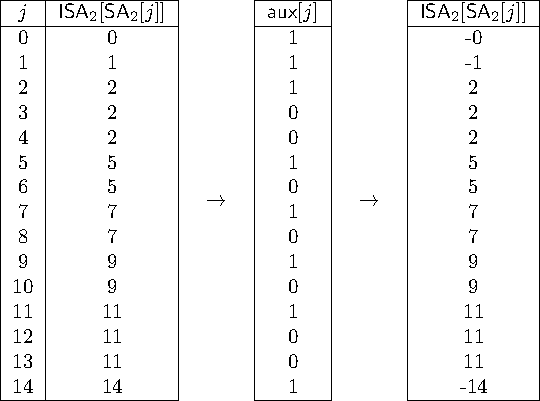
\includegraphics[scale=1]{kapitel/saca_algorithmen/osipov/mark_singletons_example.pdf}
\caption{Beispiel zur parallelen Markierung von sortierten Gruppen. Wie beschrieben, werden zunächst die Indizes ermittelt, deren Rang sich von dem des Vorgängers unterscheidet. Unterscheidet dieser sich zudem noch vom Nachfolger, handelt es sich um eine fertig sortierte Gruppe.}
\label{osipov:mark}
\end{figure}

\end{center}
\subsubsection{Tupel erzeugen}
Die Erzeugung der Tupel wird in drei Schritte aufgeteilt: Zunächst prüfen wir, für welche Indizes Tupel erstellt werden müssen. Dafür schreiben wir in unser Hilfsarray $\mathsf{aux}$ an Stelle $j$ die Anzahl der erzeugten Tupel, wobei bis zu zwei Tupel (Suffix an Stelle $j$, zu sortierender Suffix $i$) erzeugt werden können. Wurde $\mathsf{aux}$ komplett befüllt, berechnen wir die exklusive Präfixsumme über alle betrachteten Suffixe dieser Iteration. Der neue Wert in $\mathsf{aux}$ gibt nun an, an welcher Stelle wir die durch Suffix $j$ generierten Tupel einfügen. Im letzten Schritt können wir die Tupel parallel erzeugen und an die entsprechende Position einfügen. 
Für die Tupel verwalten wir zur einfacheren Nutzung drei Arrays: eines für den Index, eines für den $h$-Rang und das dritte Array für den $2h$-Rang. Um die Anzahl der erzeugten Tupel zu bestimmen, benötigen wir den letzten Index in $\mathsf{aux}$. Da die Anzahl der durch den letzten Suffix erzeugten Tupel durch die Präfixsummenoperation überschrieben wird, berechnet sich die Gesamtzahl der Tupel aus dem Wert des letzten Indizes vor der Präfixsumme und dem Wert nach der Präfixsumme. Ein Beispiel hierfür ist in Abb. \ref{osipov:create} abgebildet.

Da wir für den leichteren Zugriff auf die Ränge $h$- und $2h$-Ränge separat speichern, müssten wir ein Value-Paar aus Index und $2h$-Rang für alle Tupel generieren, um den Radixsort der CUB-Library nutzen zu können, welcher nur Key-Value-Paare (und einzelne Werte) sortieren kann. Wir haben uns stattdessen dafür entschieden, die $2h$-Ränge erst nach dem Radixsort in sortierter Reihenfolge zu erzeugen, da diese Ränge erst für das Aktualisieren der Ränge benötigt werden. Wir haben für das Befüllen des Hilfsarrays und für die Erzeugung der Tupel nach der Präfixsumme zwei unabhängige Kernel-Methoden geschrieben, da die Präfixsumme einen eigenen Kernel innerhalb der CUB-Library darstellt und der Aufruf von Kernel-Methoden nur durch Host-Methoden (von der CPU aus) möglich ist. 
\begin{center}
\begin{figure}
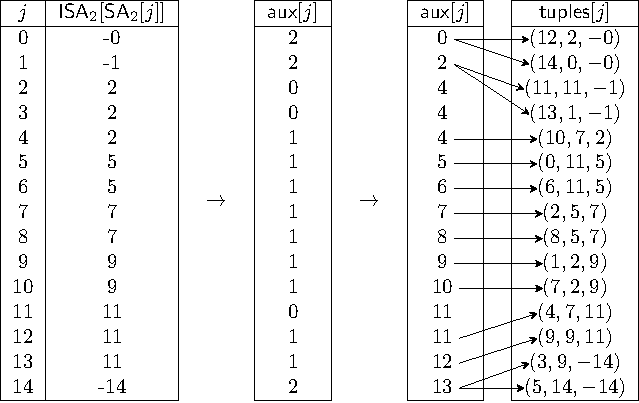
\includegraphics[scale=1]{kapitel/saca_algorithmen/osipov/create_tuple_example.pdf}
\caption{Beispiel zur parallelen Erzeugung der zu sortierenden Tupel. Zunächst werden dazu mit Hilfe des $\mathsf{aux}$-Arrays die richtigen Position für die Tupel ermittelt und diese dann von den Threads an die jeweiligen Stellen in der Tupelliste geschrieben.}
\label{osipov:create}
\end{figure}

\end{center}
\subsubsection{Ränge aktualisieren}
\begin{figure}
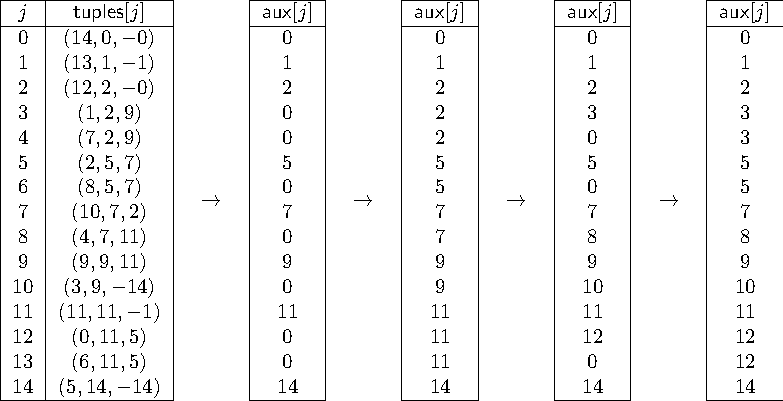
\includegraphics[scale=0.9]{kapitel/saca_algorithmen/osipov/update_ranks_example.pdf}
\caption{Beispiel zur Berechnung der neuen Ränge im Parallelen. Dazu werden, wie beschrieben, die Positionen der Gruppenköpfe im $\mathsf{aux}$ berechnet, um anschließend ins $\mathsf{ISA}$ übertragen zu werden.}
\label{osipov:update}
\end{figure}
Um die Aktualisierung der Ränge anhand der neuen Sortierung zu parallelisieren, gehen wir wie folgt vor:
Zunächst ermitteln wir die Position der Tupel, an denen eine neue $h$-Gruppe beginnt. Dafür überprüfen wir für jedes Element in der sortierten Tupelliste, ob sich der Rang von dem seines Vorgängers unterscheidet. Ist dies der Fall, schreiben wir an der korrespondierenden Stelle im $\mathsf{aux}$ den Index des Suffixes, andernfalls eine 0. Haben wir alle Tupel überprüft, berechnen wir auf dem $\mathsf{aux}$ einen Prefixscan mit Maximums-Operator. Anschließend haben wir in diesem dann zu jedem Suffix die Anfangsposition der neuen $h$-Gruppe eingetragen. 
Wir prüfen hiernach mit denselben Bedingungen wie in der sequentiellen Variante (s. Algorithmus $\ref{alg:osipov}$ Z.19 und 22), ob ein Tupel jetzt Kopf einer neuen 2$h$-Gruppe ist. Ist dies der Fall, überschreiben wir den entsprechenden Wert in $\mathsf{aux}$ mit der Differenz aus der Position des Tupels in der Liste und dem aktuellen Wert in $\mathsf{aux}$ addiert mit dem alten $h$-rank, der sich aus dem Tupel entnehmen lässt. Schließlich berechnen wir erneut auf dem $\mathsf{aux}$ einen Prefixscan mit Maximums-Operator, erhalten dadurch die neuen $2h$-Ränge und können diese dann ins $\mathsf{ISA}$ übernehmen. Ein Beispiel für dieses Vorgehen, zeigt Abb. \ref{osipov:update}.
In unserer Implementierung nutzen wir zum Befüllen des $\mathsf{aux}$ in beiden Fällen selbst implementierte Kernel Methoden, welche die vorher sortierte Liste der Tupel scannen. Für die Prefixscans nutzen wir dagegen, wie bereits bei der Tupelerzeugung, die in der CUB-Library implementierte Variante.
